\documentclass[tikz,border=8pt]{standalone}
% Shared look for every TikZ diagram. Load with \input{../../tools/tikz-style.tex}
\usepackage[T1]{fontenc}
\usepackage{lmodern}
\renewcommand{\sfdefault}{lmr}  % diagrams use the same serif as the text
\usetikzlibrary{arrows.meta, positioning, shapes.geometric, calc, fit, backgrounds}
\definecolor{cblue}{HTML}{4C78A8}
\definecolor{corange}{HTML}{F58518}
\definecolor{cgreen}{HTML}{54A24B}
\definecolor{cred}{HTML}{E45756}
\definecolor{cpurple}{HTML}{B279A2}
\definecolor{cgrey}{HTML}{6B6B6B}
\tikzset{
  every picture/.style={font=\sffamily, line width=1.2pt},
  box/.style={draw=#1, fill=#1!12, rounded corners=4pt, align=center, inner sep=7pt, minimum height=1.1cm},
  box/.default=cgrey,
  arrow/.style={-{Stealth[length=3mm]}, draw=cgrey, line width=1.4pt},
  title/.style={font=\sffamily\bfseries\Large},
  note/.style={font=\sffamily\small, text=cgrey, align=center},
}
\AtBeginDocument{\hyphenpenalty=10000 \exhyphenpenalty=10000}

\begin{document}
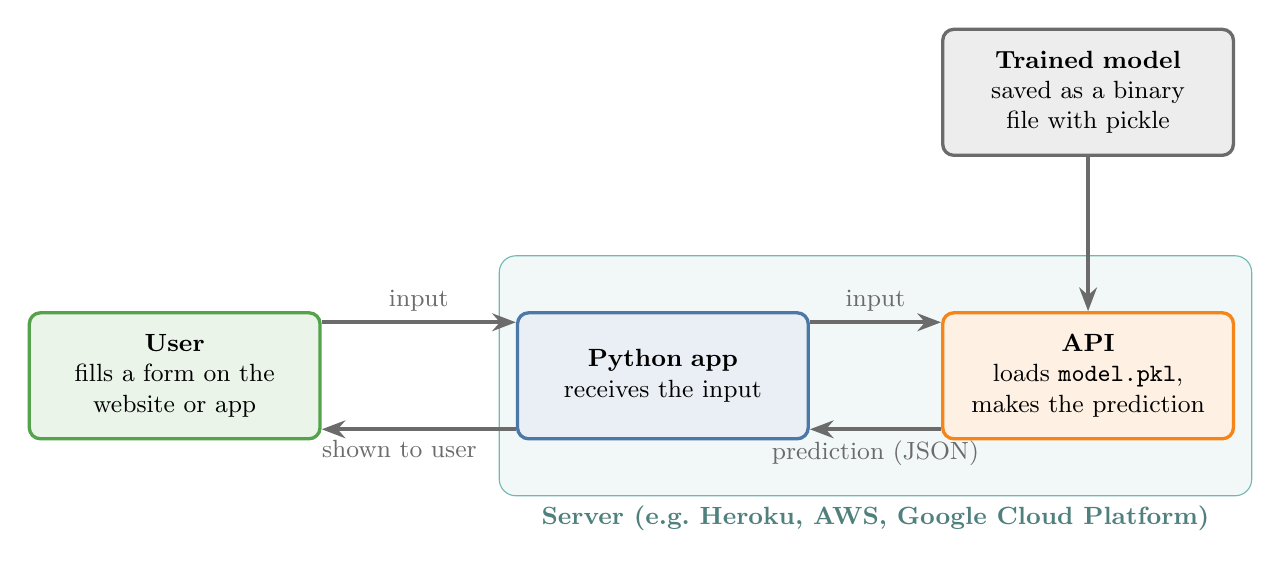
\begin{tikzpicture}
  \definecolor{cteal}{HTML}{72B7B2}
  \tikzset{st/.style={box=#1, minimum width=3.4cm, text width=3.2cm, minimum height=1.6cm, font=\small}}
  \node[st=cgreen] (u) at (0,0) {\textbf{User}\\fills a form on the website or app};
  \node[st=cblue] (p) at (6.2,0) {\textbf{Python app}\\receives the input};
  \node[st=corange] (a) at (11.6,0) {\textbf{API}\\loads \texttt{model.pkl},\\makes the prediction};
  \draw[arrow] (u.20) -- node[note, above] {input} (p.160);
  \draw[arrow] (p.20) -- node[note, above] {input} (a.160);
  \draw[arrow] (a.200) -- node[note, below] {prediction (JSON)} (p.340);
  \draw[arrow] (p.200) -- node[note, below, pos=0.6] {shown to user} (u.340);
  % the server that hosts the app and the API
  \begin{scope}[on background layer]
    \node[draw=cteal, fill=cteal!10, rounded corners=6pt, inner xsep=6pt, inner ysep=20pt, fit=(p)(a), label={[font=\small\bfseries, text=cteal!70!black]below:Server (e.g.\ Heroku, AWS, Google Cloud Platform)}] {};
  \end{scope}
  % how the model file is made
  \node[st=cgrey] (m) at (11.6,3.6) {\textbf{Trained model}\\saved as a binary file with pickle};
  \draw[arrow] (m) -- (a);
\end{tikzpicture}
\end{document}
